%! Author = joels
%! Date = 24/12/2020

\section{Values and Streams}
% You know how and where to define variables
% You can identify the type of a literal
% You know the most important operators
% You can use the basic sequence container std string
% You can read from and write to streams
% You know about the possible states of an std istream

\subsection{Variable Definitions}
\begin{itemize}
    \item Defining a variable consists of specifying its type, its variable name and its initial value. E.g. \textcolor{blue}{int x$\{$42$\}$;}
    \item Empty braces mean default initialization. E.g. \textcolor{blue}{double x$\{$$\}$;}
    \item Using = for initialization we can have the compiler determine its type. E.g. \textcolor{blue}{auto const i = 5;}
\end{itemize}

\subsubsection{Constants}
\begin{itemize}
    \item Adding the const keyword in front of the name makes the variable a single assignment variable, aka a constant. E.g. \textcolor{blue}{int const x$\{$42$\}$;}
    \SubItem{Must be initialized and immutable}
    \item Use the keyword constexpr if the variable is required to be fixed at compile time. E.g. \textcolor{blue}{double constexpr pi$\{$3.14159$\}$;}
\end{itemize}

\subsubsection{Why shoud I use const?}
\begin{itemize}
    \item A lot of code needs names for values, but often does not intend to change it
    \item It helps to avoid reusing the same variable for different purposes (code smell)
    \item It creates safer code, because a const variable cannot be inadvertently changed
    \item It makes reasoning about code easier
    \item Constness is checked by the compiler
    \item It improves optimization and parallelization (shared mutable state is dangerous)
\end{itemize}

\subsubsection{Important types for Variable}
\begin{itemize}
    \item short, int, long, long long - each also available as unsigned version
    \item bool, char, unsigned char, signed char
    \item float, double, long double
    \item void is special, it is the type with no values
    \item class defined: E.g. std::string, std::vector
\end{itemize}

\subsection{Values and Expressions}
\textbf{Integer to boolean:} 0 = False, every other value = True\\
if (a $<$ b $<$ c) $\rightarrow$ zuerst wird a $<$ b ausgewertet (true oder false). Dann wird der Boolean mit einem int (c) verglichen. Der Bool wird dafür implizit in 0 oder 1 gecastet.\\
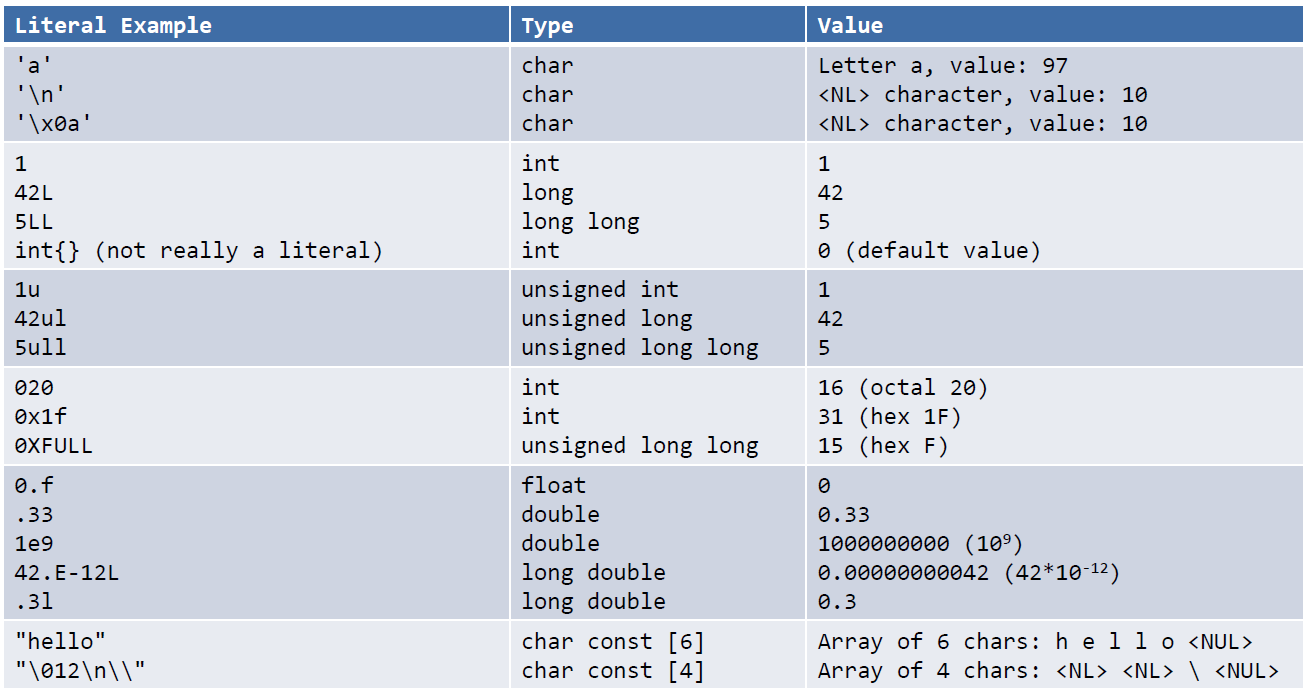
\includegraphics[scale=0.55]{literal_examples.png}

\subsection{Strings and Sequences}
std::string is C++'s type for representing sequences of char (which is often only 8 bit) and are mutable. That means, we can modify the content. (Vergleich zu Java: Dort würde ein neues String Objekt erstellt werden)\\
Grundsätzlich werden Strings also als char const[ ] abgespeichert. Mit dem namespace std::literals hat man die Option hinter dem String eine 's' anzufügen, um das Objekt effektiv als String zu speichern. z.B. \dq ab\dq s
\subsubsection{toUpper Iterator}
\begin{lstlisting}[style=frame, style= linenumbers, language=C]
void toUpper(std::string & value) {
    transform(cbegin(value), cend(value), begin(value), ::toupper);
}
\end{lstlisting}

\subsection{Input and Output Streams}
Functions taking a stream object must take it as a reference, because they provide a side effect to the stream (i.e., output characters).
\subsubsection{Reading from Input}
\begin{itemize}
    \item Reading into a std::string always works. Unless the stream is already !good() $\rightarrow$ Spaces werden übersprungen (neues String-Objekt)!
    \item Reading into other types (e.g. int) has no error recovery. A wrong input puts the stream into status fail and the characters remain in the input.
    \item Post-read check: \textcolor{blue}{if (in >> age) $\{$ ... $\}$}
    \item Multiple subsequent reads are possible: \textcolor{blue}{if (in >> symbol >> count) $\{$ ... $\}$}
    \item Remove fail flag: \textcolor{blue}{in.clear()}
    \item Ignore one char: \textcolor{blue}{in.ignore();}
    \item Helpfull for reading: \textcolor{blue}{while (in.good())} um die Leseoperationen setzen.
\end{itemize}

\subsubsection{Robust reading of an int value}
\begin{lstlisting}[style=frame, style= linenumbers, language=C]
// Use an std::istringstream as intermediate stream
int inputAge(std::istream & in)
    std::string line{}
    while (getline(in, line)) {
        std::istringstream is{line};
        int age{-1};
        if (is >> age) {
            return age;
        }
    }
    return -1;
}
/* ## dealing with invalid input ##
in.clear(); //remove fail flag
in.ignore(); // ignore one char*/

\end{lstlisting}

\subsubsection{Stream States}
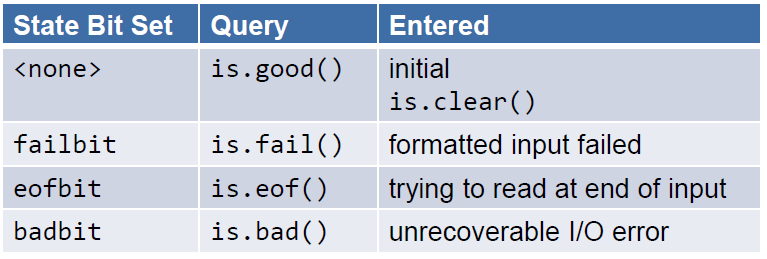
\includegraphics[scale=0.6]{stream_states}